\subsection{Brugsmønsterrealisering}

% -----------------------------------------------------------------------------------------------------------------
\subsubsection{Systemsekvensdiagram}
Et systemsekvensdiagram er et sekvensdiagram der viser systemhændelserne for ét scenarie af et brugsmønster. Diagrammet viser hvordan aktørerne interagerer med systemet for at opfylde brugsmønstret. Diagrammet viser systemet som en ‘black box’, hvilket betyder at man ikke kan se
hvad der sker inde i systemet, man kun hvad der sker udenfor systemet. På diagrammet ses det, hvordan aktørerne genererer systembegivenheder og hvad systemets output er. Ydermere viser diagrammet den ‘tidslinje’ begivenhederne sker i. \\
\myworries{Et eksempel på et systemsekvensdiagram kan ses nedenfor.} \\


\begin{figure}[H]
\centering
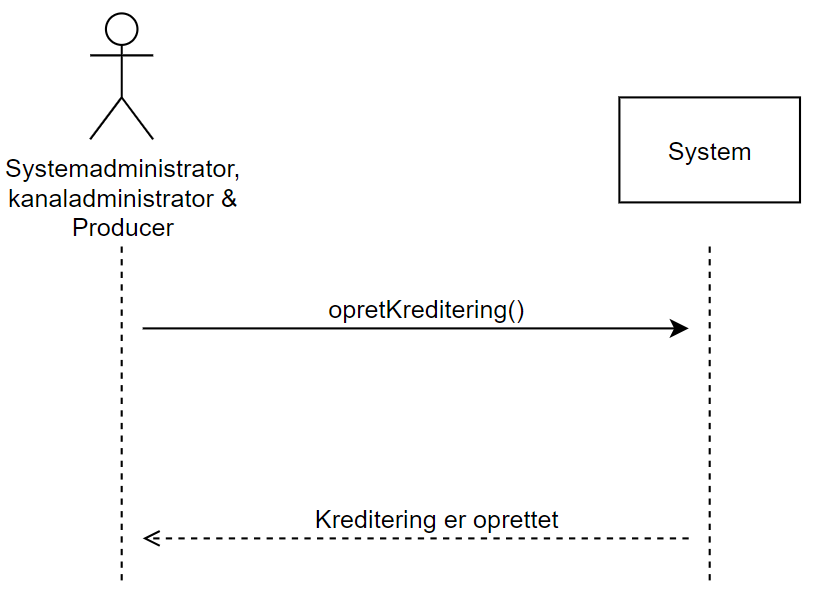
\includegraphics[scale=0.4]{figures/systemsekvensdiagrammer/opretKreditering.PNG}
\caption{Systemsekvensdiagram for "Opret Kreditering"}
\label{fig:systemsekvensdiagram_opretKreditering}
\end{figure}


\myworries{Her kan vi se, at aktøren (Systemadministrator, kanaladministrator eller Producer) kalder metoden opretKreditering ind til systemet, som returnerer at en kreditering er blevet oprettet. Vi kan altså ikke se hvordan krediteringen bliver oprettet, og vi holder os dermed til hvad der sker uden for systemet. Ud over det ovenstående (system)sekvensdiagram har vi valgt at medtage systemsekvensdiagrammer for \textit{godkendKreditering}, \textit{opretProducer}, \textit{sePersonInfo} og \textit{læsKreditering}. } \\

\myworries{Efter systemsekvensdiagrammerne er lavet, finder man de operationer systemsekvensdiagrammet kræver. Vi kigger altså her ikke længere blot udenfor systemet, men ser på præcis hvordan 'flowet' for brugsmønstret udvikles. Til dette skal vi kigge på kontrakter for systemfunktioner.} \\

\myworries{ Indsæt tekst om hvilke systemsekvensdiagrammer vi har valgt at medbringe her i teksten, hvorfor og at de andre kan findes i bilag :-) - Sammenkobel den her tekst med den tekst der er i brugsmønsterrealisering - kechr  } \\

\begin{figure}[H]
\centering
\includegraphics[scale=0.43]{figures/systemsekvensdiagrammer/læsKreditering.PNG}
\caption{Systemsekvensdiagram for "Læs kreditering"}
\label{fig:read_credit}
\end{figure}


% -----------------------------------------------------------------------------------------------------------------
\subsubsection{Kontrakter for systemfunktioner}
En systemoperationskontrakt beskriver en operations ansvar, altså hvad en operation har forpligtet sig til. Kontrakten lægger vægt på hvad en operation ændrer på, og ikke på hvordan det ændre sig. En kontrakt kan derfor anses som værende en formel beskrivelse af en operation.\\
Systemoperationskontrakten indeholder navnet på operationen, krydsreferencer til de relevante brugsmønstre, beskrivelse af ansvaret, det output operationen genererer, samt pre- og postkonditioner for operationen. \\
Pre- og postkondinitionerne er stilbilleder af systemet på det givne tidspunkt operationen bliver kaldt. De beskriver altså systemets tilstand før og efter at operationen har kørt. Postkonditioner skal altid noteres i datid, som f.eks. “Købet blev foretaget”, da det er en ting der er sket, og ikke sker.\\

\noindent
\myworries{Det er valgt at lave operationskontrakter for de samme operationer som ved systemsekvensdiagrammerne, da disse operationer viser essensen af den logik der skal implementeres.} \\

\myworries{Skriv dette om - Sammenkoble med den tekst der står under systemsekvensdiagrammer -- Eventuelt skriv det under 10. brugsmønsterrealisering, at vi har valgt at arbejde med de brugsmøsnter/operationer/we vi har - begrund uddybende - kechr}

% Skal "overskriften" ikke bare fjernes fra nedenstående tabeller? - kechr
% Skal vi bare indsætte en enkelt operationskontrakt, og smide resten i bilagene?

%------------------------ Læs krediteringer -------------------------------
\begin{table}[H]
    \begin{tabularx}{\textwidth}{|p{4cm}|X|}
        \hline
        \multicolumn{2}{|X|}{\textbf{Læs Kreditering}}\\ 
        \hline
        \textbf{System operation}       & \textbf{læsKreditering} \\ \hline
        \textbf{Krydshenvisning}        & Use case: Læs kreditering \\ \hline
        \textbf{Ansvar}                 & At vise eksisterende krediteringer, hvis følgende betingelser er sande \\ 
                                        & \\
                                        & \quad 1. Den søgte kreditering findes i systemet\\
                                        & \\
                                        & Hvis ikke overstående er sande, skal det sendes en besked til brugeren at den søgte kreditering ikke findes i systemet\\\hline
        \textbf{Output}                 & 1. Krediteringen vises\\ 
                                        & Alternativt: Besked sendt ud til brugeren\\ \hline
        \textbf{Prækonditioner}         & Ingen \\ \hline
        \textbf{Postkonditioner}        & En kreditering vil blive vist \\ \hline
    \end{tabularx}
    \caption{Systemfunktionskontrakt 'læsKreditering'}
    \label{tab:kontrakter_læs_kreditering}
\end{table}


%------------------------ Opret kreditering -------------------------------
\begin{table}[H]
    \begin{tabularx}{\textwidth}{|p{4cm}|X|}
        \hline
        \multicolumn{2}{|X|}{\textbf{Opret kreditering}}\\
        \hline
        \textbf{System operation}       & \textbf{opretKreditering} \\ \hline
        \textbf{Krydshenvisning}        & Use case: Opret Kreditering \\ \hline
        \textbf{Ansvar}                 & At oprette krediteringer og sende den videre til godkendelse hvis prækonditionen er opfyldt, og                                       følgende betingelser er sande: \\
                                        & \\
                                        & \quad 1. Minimumskravene er opfyldt\\
                                        & \quad 2. Alle oplysninger er indtastet korrekt \\
                                        & \\
                                        & Hvis ikke ovenstående er sande, oprettes krediteringen ikke, og brugeren bliver informeret herom \\ \hline
        \textbf{Output}                 & \quad 1. Produceren får besked om krediteringen er oprettet \\ 
                                        & \quad 2. System- og/eller kanaladministrator får besked om en nyoprettet kreditering \\\hline
        \textbf{Prækonditioner}         & Logget ind som kanal- eller systemadministrator \\ \hline
        \textbf{Postkonditioner}        & En ny kreditering er oprettet i systemet \\ \hline
    \end{tabularx}
    \caption{Systemfunktionskontrakt 'Opret kreditering'}
    \label{tab:kontrakter_opret_kreditering}
\end{table}


%------------------------ Opret producer -------------------------------
\begin{table}[H]
    \begin{tabularx}{\textwidth}{|p{4cm}|X|}
        \hline
        \multicolumn{2}{|X|}{\textbf{Opret producer}}\\
        \hline
        \textbf{System operation}       & \textbf{opretProducer} \\ \hline
        \textbf{Krydshenvisning}        & Use case: Opret producer \\ \hline\textbf{}
        \textbf{Ansvar}                 & At oprette en producer, hvis prækonditionen er opfyldt og følgende betingelser er sande: \\ 
                                        & \\ 
                                        & \quad 1. Produceren eksisterer ikke i systemet i forvejen \\
                                        & \quad 2. Alle oplysninger er indtastet korrekt \\
                                        & \\
                                        & Derefter give brugeren besked om det lykkedes at oprette en producer eller ej \\\hline
        \textbf{Output}                 & Besked om der er blevet oprettet en producer eller ej \\ \hline
        \textbf{Prækonditioner}         & Vedkommende der prøver at oprette en producer skal være logget ind som 'Kanal- eller                                                  Systemadministrator' \\ \hline
        \textbf{Postkonditioner}        & En ny producer er oprettet i systemet \\ \hline
    \end{tabularx}
    \caption{Systemfunktionskontrakt 'Opret producer'}
    \label{tab:kontrakter_opret_producer}
\end{table}


%------------------------ Se Personinformationer -------------------------
\begin{table}[H]
    \begin{tabularx}{\textwidth}{|p{4cm}|X|}
        \hline
        \multicolumn{2}{|X|}{\textbf{Se Personinformationer}}\\
        \hline
        \textbf{System operation}       & \textbf{sePersonInfo} \\ \hline
        \textbf{Krydshenvisning}        & Use case: Se personinformation \\ \hline
        \textbf{Ansvar}                 & At vise respektive persondata om den søgte person, hvis prækonditionen og betingelsen er opfyldt:\\
                                        & \\
                                        & \quad 1. Personen er logget ind som enten producer, kanal- eller systemadministrator\\
                                        & \\
                                        & Hvis ikke overstående er opfyldt, vises ikke personfølsomme informationer, som navn, roller i film/serier som personen har medvirket i\\ \hline
        \textbf{Output}                 & Viser en information om en person \\ \hline
        \textbf{Prækonditioner}         & Person er fundet i systemet \\ \hline
        \textbf{Postkonditioner}        & Alt efter ens rolle i systemet vil forskelligt data blive vist. Begrænset hvis man er besøgende, alt hvis man er producer, royalty bruger, kanal- og systemadministrator \\ \hline
    \end{tabularx}
    \caption{Systemfunktionskontrakt 'se personinformationer'}
    \label{tab:kontrakter_se_personinformationer}
\end{table}

%------------------------ Godkend nye krediteringer -------------------------
\begin{table}[H]
    \begin{tabularx}{\textwidth}{|p{4cm}|X|}
        \hline
        \multicolumn{2}{|x|}{\textbf{Godkend ny kreditering}}\\
        \hline
        \textbf{System operation}       & \textbf{godkendKreditering} \\ \hline
        \textbf{Krydshenvisning}        & Use case: Godkend Kredtiteringer \\ \hline
        \textbf{Ansvar}                 & At godkende eller afvise nye krediteringer hvis prædonditionerne er sande og betingelsen opfyldt:  \\ 
                                        & \\
                                        & \quad 1. En kreditering er oprettet af en producer \\
                                        & \\
                                        & Hvis ikke ovenstående er opfyldt, vil der ikke blive vist nye krediteringer til godkendelse. \\ \hline
        \textbf{Output}                 & Besked om krediteringen er godkendt \\ \hline
        \textbf{Prækonditioner}         & 1. Er logget ind som system- eller kanaladministrator \\ \hline
        \textbf{Postkonditioner}        & Krediteringen er enten godkendt eller afvist og den ansvarlige producer er bliver informeret herom \\ \hline
    \end{tabularx}
    \caption{Systemfunktionskontrakt 'Godkend nye krediteringer'}
    \label{tab:kontrakter_Godkend_nye_krediteringer}
\end{table}



% -----------------------------------------------------------------------------------------------------------------
\subsubsection{Operationssekvensdiagram}
Operationssekvensdiagrammet viser systemet som en ”white box”, hvor man kan se hvad der sker inde i systemet. Sekvensdiagrammet bruges til at identificere systemfunktioner, da de begivenheder der vises i diagrammet er de funktioner systemet skal indeholde. Et eksempel på et operationssekvensdiagram for "Læs Kreditering" kan ses nedenfor.

\begin{figure}[ht] % <--- HUSK AT ÆNDRE MIG :-)
\centering
\includegraphics[scale=1]{figures/Operationssekvensdiagrammer/læsKreditering.pdf}
\caption{Operationssekvensdiagram: Læs kreditering}
\label{fig:op_read_credit}
\end{figure}

% -----------------------------------------------------------------------------------------------------------------
\subsubsection{Revurderet analysemodel}

\myworries{De fundne metoder tilføjer vi til analysemodellen vi lavede tidligere.} \\
% ---------------------------------------------------------------INDSÆT MODEL
\myworries{Da der ikke er fundet nogle nye klasser under brugsmønsterrealiseringen, opdateres modellen ikke yderligere. } \\